\documentclass[letter,12pt]{article}
%There are several packages which I use throughout the file.  Not all will be helpful in every document, but the first several are almost always useful.  I try to note the relevant heading material in the body below as I use it.  

% Important packages
\usepackage{latexsym}
\usepackage{amsmath}
\usepackage{amssymb}
\usepackage{natbib}

% More packages
\usepackage{amsthm}
\usepackage{graphicx}
\usepackage{xcolor}
\usepackage{verbatim}
\usepackage{listings}
\usepackage{tikz,times}
\usepackage[latin1]{inputenc}
\usepackage[right=1in,bottom=1in,left=1in,top=1in]{geometry}
\usepackage{rotating}
\usepackage{cancel}
\usepackage{setspace}

\newtheorem{theorem}{Theorem}
\newtheorem{definition}{Definition}
\newtheorem{proposition}{Proposition}
\newtheorem{corollary}{Corollary}

\lstset{breaklines=true, backgroundcolor=\color{blue!10},language=,breakindent=0pt}

\newcommand{\hilight}[1]{\colorbox{yellow}{#1}}

\usetikzlibrary{calc, matrix, positioning, arrows, mindmap, backgrounds}


\title{A \LaTeX\ Problem Set Template (With Solutions)}
\author{Garrett Darl Lewis\thanks{Department of Politics, Princeton University  130 Corwin Hall, Princeton, NJ 08544-1012  E-mail: glewis@princeton.edu, }\\ Department of Politics\\ Princeton University}
\date{\today}

%\doublespacing



%%%%%%%%%%%%%%%%%%%%%%%%%%%%%%%%%%%%%%%%%%%%%%%%%%%%%%%%%



\begin{document}
\maketitle
\tableofcontents

\begin{abstract}
This document demonstrates the use of many features which are likely to be useful in preparing \LaTeX\ documents.  There are sections demonstrating basic text, math, code, and images (both internally and externally produced).  I also throw in little features such as \textbf{bold} and \textit{italic} sections, which you can find the code for within the \TeX\ file.  If there are things that you would like to see added, let me know.  This is just a quick collection of features I thought to throw together in an evening.  Of course, there are any number of websites (and presumably books, but who are we kidding) which go through this same material and heaps more.  This document merely attempts to demonstrate how many of the common features available in this typesetting environment may be applied in context.  For the full range of capabilities, I highly recommend using online resources which include the complete documentation for these commands.  Whenever I introduce a new feature, though, I include a section in blue which demonstrates the code used to produce the output in question.  If you are completely new to \LaTeX , you will want to download some software to begin.  I use \textbf{TeXworks}, but that is only one of many options out there.  Many have a stronger UI than mine, and the most bare-bones versions have no GUI.  
\end{abstract}

%\newpage



%%%%%%%%%%%%%%%%%%%%%%%%%%%%%%%%%%%%%%%%%%%%%%%%%%%%%%%%%



\section{The Main Body}\label{mainbody}

\begin{lstlisting}
\section{The Main Body}\label{mainbody}
\end{lstlisting}

% Packages
%\usepackage{latexsym, amsmath, amssymb, verbatim, natbib}

The following code is sufficient to produce a basic document.  In the preamble, it defines the type of document being created (\emph{documentclass}), any special packages that might be required to compile the document (\emph{usepackage}), as well as a statement of the title and author of the work.  As I introduce more sophisticated capabilities of the software, I will also discuss more packages and settings that can be called in the preamble when they are needed.  

At the end of the preamble, the command, \lstinline!\begin{document}!, begins the main body.  After this command, I tell the software to include a title, table of contents, and an abstract.  I then insert the main text, and finally call a bibliography using references written to the file, \emph{BiblioTemp.bib}.  The command, \lstinline!\end{document}! ends the document.  After saving, I typically run three commands in my compiler to prepare the document and ensure that all of the auxiliary files have been properly updated.  These three commands are \emph{pdfLaTeX}, \emph{MakeIndex}, and \emph{BibTeX}.  It is generally not necessary to run all three, but as it it better than spending hours on end trying to figure out why your document is not compiling properly, only to find out that your \emph{*.bbl} file was out of date.  

\begin{lstlisting}
\documentclass[letter,12pt]{article}
%There are several packages which I use throughout the file.  Not all will be helpful in every document, but the first several included here are almost always useful.  I try to note the relevant heading material in the body below as I use it.  

% Important packages
\usepackage{latexsym, amsmath, amssymb, amsthm, natbib, setspace}

% Define the title, \&c
\title{My Title}
\author{Me\thanks{Department of Politics, Princeton University}\\ Department of Politics\\ Princeton University}
\date{\today}

\doublespacing 	% Use double spacing

\begin{document}	% Begin the body
\maketitle 		% Generate the title
\tableofcontents 	% Generate a ToC

\begin{abstract}
Put your abstract here! 
\end{abstract}

\section{The Body}
Hello World!

\newpage 	% Skip to the next page
\bibliography{BiblioTemp} % Insert a bibliography
\end{document}
% Everything down here is ignored
\end{lstlisting}



%%%%%%%%%%%%%%%%%%%%%%%%%%%%%%%%%%%%%%%%%%%%%%%%%%%%%%%%%%



\subsection{Text}\label{text}

Basic text is pretty easy.  Just define your document class, open your document, and start typing, maybe adding a chapter or section along the way.  However that's pretty boring, especially if you're not an English major and have to use things like, \emph{you know}, \textbf{MATH}.  Let's look at some of the options\dots\footnote{I want to quickly point out a few features that can drive someone crazy if they are not paying attention.  Many symbols, such as \&, \textasciitilde, and \textbackslash\ require special notation in \LaTeX , since the symbols themselves have certain meaning in the software.  Make sure you proofread your finished document--esp. where you are likely to use symbols--to ensure that there are no odd missing items or strange additions.}  

In the previous paragraph, we saw features like italics and bold face type, as well as an ellipsis and a footnote.  These are typeset as, 
\begin{lstlisting}
...have to use things like, \emph{you know}, \textbf{MATH}.  Let's look at some of the options\dots\footnote{I want to quickly point out a few features that can drive someone crazy if they are not paying attention.  Many symbols, such as \&, \textasciitilde, and \textbackslash\ require special notation in \LaTeX , since the symbols themselves have certain meaning in the software.  Make sure you proofread your finished document--esp. where you are likely to use symbols--to ensure that there are no odd missing items or strange additions.}
\end{lstlisting}



%%%%%%%%%%%%%%%%%%%%%%%%%%%%%%%%%%%%%%%%%%%%%%%%%%%%%%%%%%



\subsection{References}

\begin{lstlisting}
\subsection{References}
\end{lstlisting}

In many instances, you want to refer to something that is in a different section of your document or even in a different document.  To do the former, you need only label your sections, equations, theorems, \&c. as you go along, just as I did here in Section \ref{text}.  By default, numbers are used to reference items, with a unique counter for each environment (sections, equations, \&c.), but there are ways to change that.  In sections \ref{theorem} and \ref{math}, I mention \emph{counter} tools and the \emph{tag} feature.  

\begin{lstlisting}
...label your sections, equations, theorems, \&c. as you go along, just as I did here in Section \ref{text}...
\end{lstlisting}

And of course there is the question of references to other works.  The most useful commands for that are \emph{cite} and \emph{citep} \citep{Lewis14} (Ignore the fact that I'm citing myself to back up this claim).  The bibliography style I use here is \emph{JPE} and I compile my references using $\mathrm{B{\scriptstyle{IB}}}$\TeX.  Of course, different journals and subfields may prefer different formats from these presented here, but hopefully this will get you off the ground.  

\begin{lstlisting}
...useful commands for that are \emph{cite} and \emph{citep} \citep{Lewis14}...
\end{lstlisting}

\begin{lstlisting}
...I compile my references using $\mathrm{B{\scriptstyle{IB}}}$\TeX...
\end{lstlisting}

When referencing you bibliography, the program will skip over citations if it they cannot be found in a \emph{*.bib} file (that has also been appropriately compiled using $\mathrm{B{\scriptstyle{IB}}}$\TeX).  If this happens, you will receive a question mark in lieu of the citation.  Luckily, the \emph{*.bib} file is easy to assemble, since it is little more than a list of all your sources:  

\begin{lstlisting}
@ARTICLE{Lewis14,
   AUTHOR  = {Lewis, Darl},
   TITLE   = {A \LaTeX Template},  
   YEAR    = {2014},
   JOURNAL = {A Journal},
   VOLUME  = {1},
   NUMBER  = {1},
   PAGES   = {1-12}
}
%
@BOOK{Lewis14a,
   AUTHOR  = {Lewis, Darl},
   TITLE   = {A \LaTeX Book},  
   YEAR    = {2014},
   PUBLISHER = {My Computer},
   ADDRESS  = {NJ},
}
%
@INCOLLECTION{Lewis14b,
   AUTHOR  = {Lewis, Darl},
   TITLE   = {Another \LaTeX Template},  
   YEAR    = {2014},
   EDITOR = {Lewis, Darl},
   BOOKTITLE  = {Another \LaTeX Book},
   PUBLISHER = {My Computer},
   ADDRESS  = {NJ},
}
\end{lstlisting}

To insert the list of references at the end of your document, simply define the bibliography style and call the bibliography before you end the document.  The \emph{nocite} option allow the software to include references in the works cited section whether or not thay have been cited within the document.  

\begin{lstlisting}
\bibliographystyle{jpe}
\nocite{*}
\bibliography{BiblioTemp}
\end{lstlisting}



%%%%%%%%%%%%%%%%%%%%%%%%%%%%%%%%%%%%%%%%%%%%%%%%%%%%%%%%%%



\subsection{Theorems, \&c.}\label{theorem}

There are a few environments readily available for writing theorems and proofs and the like, but sometimes you have to define your own.  Luckily, that's easy to do.  In the preamble of my document, I have defined four environments, \emph{Theorem}, \emph{Definition}, \emph{Proposition}, and \emph{Corollary}, using these commands: 

\begin{lstlisting}
\newtheorem{theorem}{Theorem}
\newtheorem{definition}{Definition}
\newtheorem{proposition}{Proposition}
\newtheorem{corollary}{Corollary}
\end{lstlisting}

\LaTeX\ counts each environment separately unless specified otherwise using any of the \emph{counter} tools such as \emph{addtocounter} and \emph{newcounter}.  



\begin{theorem}
All governments are unjust.
\end{theorem}

\begin{proof}
Consider an arbitrary government. Since it is arbitrary, it is obviously unjust.  The assertion being correct for an arbitrary government, it is thus true for all governments.
\end{proof}

\begin{lstlisting}
\begin{theorem}
All governments are unjust.
\end{theorem}

\begin{proof}
Consider an arbitrary government. Since it is arbitrary, it is obviously unjust.  The assertion being correct for an arbitrary government, it is thus true for all governments.
\end{proof}
\end{lstlisting}

\begin{definition}[Circular Definition]
See: \emph{Definition, Circular}.
\end{definition}

\begin{lstlisting}
\begin{definition}[Circular Definition]
See: \emph{Definition, Circular}.
\end{definition}
\end{lstlisting}

\begin{proposition} 
Will you marry me?
\end{proposition}

\begin{corollary}
And sign a prenup.
\end{corollary}

\begin{lstlisting}
\begin{proposition} 
Will you marry me?
\end{proposition}

\begin{corollary}
And sign a prenup.
\end{corollary}
\end{lstlisting}

\begin{proposition}[Humor]
This section has some really bad humor.
\end{proposition}

\begin{proof}
Reread the section.  The rest is trivial. 
\end{proof}

\begin{lstlisting}
\begin{proposition}[Humor]
This section has some really bad humor.
\end{proposition}

\begin{proof}
Reread the section.  The rest is trivial. 
\end{proof}
\end{lstlisting}



%%%%%%%%%%%%%%%%%%%%%%%%%%%%%%%%%%%%%%%%%%%%%%%%%%%%%%%%%%



\subsection{Math}\label{math}

The value of \LaTeX\ becomes most apparent when writing equations.  After a while, it becomes very easy to simply type equations as you go in a way that does not accrue with many other software platforms.  Most mathematical symbols are simply a \textbackslash\ followed by the name of the symbol, and most of the common structures you are likely to encounter are designed to be implemented with relative ease and flexibility.  If you want to write an inline equation, just use the \$ like this $a+b=c$.  

\begin{lstlisting}
...If you want to write an inline equation, just use the \$ like this $a+b=c$.
\end{lstlisting}

If you want to to write something longer or make it more visible by pulling it out of the text, though, use the \emph{equation} environment:

\begin{equation}
\mathrm{e}^{i\pi}+1=0
\end{equation}

\begin{lstlisting}
\begin{equation}
\mathrm{e}^{i\pi}+1=0
\end{equation}
\end{lstlisting}

If you don't want to attach a number, there are several options.  I usually just go with this one...

\[
\rho\left(\frac{\partial \mathbf{v}}{\partial t}+\mathbf{v}\cdot\nabla\mathbf{v}\right)=-\nabla p+\nabla\cdot\mathbf{T}+f
\]

\begin{lstlisting}
\[
\rho\left(\frac{\partial \mathbf{v}}{\partial t}+\mathbf{v}\cdot\nabla\mathbf{v}\right)=-\nabla p+\nabla\cdot\mathbf{T}+f
\]
\end{lstlisting}

And of course, if you want to name a multiline equation,

\begin{equation}\tag{Bad Math}
\begin{split}
a+b&=c \\
2(a+b)-(a+b)&=2c-c \\
2a+2b-2c&=a+b-c \\
2(a+b-c)&=a+b-c \\
2&=1
\end{split}
\end{equation}

\begin{lstlisting}
\begin{equation}\tag{Bad Math}
\begin{split}
a+b&=c \\
2(a+b)-(a+b)&=2c-c \\
2a+2b-2c&=a+b-c \\
2(a+b-c)&=a+b-c \\
2&=1
\end{split}
\end{equation}
\end{lstlisting}

Note the use of the \emph{split} environment and the \& to align equations in this system.  

There are other ways of separating an equation into multiple lines with slightly varying effects.  These include, \emph{multline}, \emph{align}, \emph{gather}, and \emph{eqnarray}, among others.  

Sometimes you may want to nest a few related equations under one number.  Try this:

\begin{subequations}\label{mygrp}
\begin{align}
a+b&=c \label{firstgrp}\\
c&=d+e \\
d&=f+g \\
e&=h+i 
\end{align}
\end{subequations}

\begin{lstlisting}
\begin{subequations}\label{mygrp}
\begin{align}
a+b&=c \label{firstgrp}\\
c&=d+e \\
d&=f+g \\
e&=h+i 
\end{align}
\end{subequations}
\end{lstlisting}

If you label them properly, you can easily refer back to previous equations like \eqref{mygrp}.  That makes it easy to talk about how similar \eqref{firstgrp} is to the first equation I presented here in Section \ref{math}.

\begin{lstlisting}
If you label them properly, you can easily refer back to previous equations like \eqref{mygrp}.
\end{lstlisting}

For more on mathematical features and symbols, I will refer you to a well-written document in \cite{Downes02}, which offers a quick run-down of the capabilities of the software.  For a comprehensive list of symbols available, both in the equation environment and the text environment, see \cite{Pakin09}.  



%%%%%%%%%%%%%%%%%%%%%%%%%%%%%%%%%%%%%%%%%%%%%%%%%%%%%%%%%%



\subsection{Code}

Sometimes you may want to put code directly into your document.  The easiest way is with the \emph{verbatim} package, something you will see in several of the images that come later in this document.  

\begin{verbatim}
% Don't do this!
i=1
while i>0
    	i++
end;
\end{verbatim}

\begin{lstlisting}
\begin{verbatim}
% Don't do this!
i=1
while i>0
    	i++
end;
\end{verbatim}
\end{lstlisting}

Of course, with \emph{verbatim}, you're not restricted to writing code.  Any text is fine as long as you're willing to live with that plain ASCII feel.  On the other hand, if you are looking for something more sophisticated to insert plain text or code, as I have been doing throughout this document, you may prefer to use the more-versatile \emph{listings} package, which has been explicitly designed for inserting code into \LaTeX\ files.  To implement that package, simply replace the word, \emph{verbatim}, in the previous block of code with the word, \emph{lstlisting}.  Throughout this document, I have use the following settings, defined in the preamble:

\begin{lstlisting}
\lstset{breaklines=true, backgroundcolor=\color{blue!10},language=,breakindent=0pt}
\end{lstlisting}




%%%%%%%%%%%%%%%%%%%%%%%%%%%%%%%%%%%%%%%%%%%%%%%%%%%%%%%%%%
%%%%%%%%%%%%%%%%%%%%%%%%%%%%%%%%%%%%%%%%%%%%%%%%%%%%%%%%%%




\section{Tables}

Tables in \LaTeX, like everything else, take some getting used to, but they can come out very nicely once you've taken the time to assemble them.  Many statistical packages (including \textbf{Stata} and \textbf{R}) also offer macros which will output data in \LaTeX\ format to save you the trouble.  By default, the software places tables where they best fit in the text, which is not always precisely where they are written in the source.

\begin{table}\caption{The auto data\label{auto}}
\begin{center}
\begin{tabular}{l*{2}{rr}}
\hline
		&\multicolumn{2}{c}{Model 1}	&\multicolumn{2}{c}{Model 2}\\
		& Coef.	& $p$-value		& Coef.	& $p$-value\\
\hline\\[-1ex] 
Weight (lbs.)	& 1.747	& .008		& 4.614	& .000\\
Mileage (mpg) & --.050	& .567		& .263	& .020\\
Foreign*Mileage & 		& 			& --.307	& .006\\
Foreign car type& 		& 			& 11.240	& .000\\
Constant 	& 1.946	& .590		& --14.450	& .002\\
\hline
Adj. $R^2$ 	& .273	& 			& .526	& \\
No. of cases 	& 74		& 			& 74		& \\
\hline
\small\textit{Source:} auto.dta
\end{tabular}
\end{center}
\end{table}

\begin{lstlisting}
\begin{table}\caption{The auto data\label{auto}}
\begin{center}
\begin{tabular}{l*{2}{rr}}
\hline
&\multicolumn{2}{c}{Model 1}	&\multicolumn{2}{c}{Model 2}\\
& Coef.	& $p$-value		& Coef.	& $p$-value\\
\hline\\[-1ex] 
Weight (lbs.)		& 1.747 & .008 & 4.614   & .000\\
Mileage (mpg) 		& -.050 & .567 & .263    & .020\\
Foreign*Mileage 	&       &      & -.307   & .006\\
Foreign car type	&       &      & 11.240  & .000\\
Constant 		& 1.946 & .590 & -14.450 & .002\\
\hline
Adj. $R^2$ 		& .273  &      & .526 & \\
No. of cases 		& 74    &      & 74   & \\
\hline
\small\textit{Source:} auto.dta
\end{tabular}
\end{center}
\end{table}
\end{lstlisting}


That table wasn't very complicated.  Let's look at some other features now which add a little fun to to the process.  Here I am going to write a table which has been turned sideways (ostensibly because it fits better in landscape mode) using the \emph{rotating} package.  To avoid interfering with the surrounding text, this table is placed at the end of the document.  Rewriting this second table for statistical data would not be a challenging task.  

% Pakages
%\usepackage{rotating}L

\begin{sidewaystable}[h] 
\caption{Performance After Post Filtering} % title name of the table 
\centering % centering table 
\begin{tabular}{l c c rrrrrrr} % creating 10 columns 
\hline\hline \\[-1ex]% inserting double-line 
 Audio 			&Audibility 			& Decision 	&\multicolumn{7}{c}{Sum of Extracted Bits} \\ [0.5ex] 
\hline % inserts single-line 
 				& 				&soft 		&1 	& $-1$ 	& 1 	& 1 	& $-1$ 	& $-1$ 	& 1 \\[-1ex] 
\raisebox{1.5ex}{Police} 	& \raisebox{1.5ex}{5}	&hard 	& 2 	& $-4$ 	& 4 	& 4 	& $-2$ 	& $-4$ 	& 4 \\[1ex] 
 				& 				&soft 		& 1 	& $-1$ 	& 1 	& 1 	& $-1$ 	& $-1$ 	& 1 \\[-1ex] 
\raisebox{1.5ex}{Beethoven} & \raisebox{1.5ex}{5}& hard 	&8 	& $-8$ 	& 2 	& 8 	& $-8$ 	& $-8$ 	& 6 \\[1ex] 
 				& 				&soft 		& 1 	& $-1$ 	& 1 	& 1 	& $-1$ 	& $-1$ 	& 1 \\[-1ex] 
\raisebox{1.5ex}{Metallica} & \raisebox{1.5ex}{5}	& hard 	&4 	& $-8$ 	& 8 	& 4 	& $-8$ 	& $-8$ 	& 8 \\[1ex] 
\hline % inserts single-line 
\end{tabular} 
\label{tab:LPer} 
\end{sidewaystable} 

\begin{lstlisting}
\begin{sidewaystable}[h] 
\caption{Performance After Post Filtering} % title of the table 
\centering % centering table 
\begin{tabular}{l c c rrrrrrr} % creating 10 columns 
\hline\hline \\[-1ex]% inserting double-line 
 Audio &Audibility & Decision &\multicolumn{7}{c}{Sum of Extracted Bits} \\ [0.5ex] 
\hline % inserts single-line 
 			& &soft &1 & $-1$ & 1 & 1 & $-1$ & $-1$ & 1 \\[-1ex] 
\raisebox{1.5ex}{Police} & \raisebox{1.5ex}{5}&hard & 2 & $-4$ & 4 & 4 & $-2$ & $-4$ & 4 \\[1ex] 
 			& &soft &1 & $-1$ & 1 & 1 & $-1$ & $-1$ & 1 \\[-1ex] 
\raisebox{1.5ex}{Beethoven} & \raisebox{1.5ex}{5}& hard &8 & $-8$ & 2 & 8 & $-8$ & $-8$ & 6 \\[1ex] 
 			& &soft & 1 & $-1$ & 1 & 1 & $-1$ & $-1$ & 1 \\[-1ex] 
\raisebox{1.5ex}{Metallica} & \raisebox{1.5ex}{5}& hard &4 & $-8$ & 8 & 4 & $-8$ & $-8$ & 8 \\[1ex] 
\hline % inserts single-line 
\end{tabular} 
\label{tab:LPer} 
\end{sidewaystable} 
\end{lstlisting}

Of course, sometimes you may have a desire to draw tables for not-statistical purposed.  Below are several small tables with different features that you may find helpful.  These examples use the \emph{color} and \emph{cancel} packages, as well as a new command, \emph{hilight}, defined in the preamble:  

\begin{lstlisting}
\newcommand{\hilight}[1]{\colorbox{yellow}{#1}}
\end{lstlisting}

% Packages
%\usepackage{cancel, color}

%\quad creates a box
%\cline{x-y} creates a vertical line over columns x to y
%\vline is a vertical line in a column

\begin{enumerate}
\item Prisoner's Dilemma 
\setlength{\arraycolsep}{0pt}
\[
\begin{array}{cccccc}
 & & \quad L \quad & & \quad R \quad & \\[.2ex] 
\cline{3-5} T \quad & \vline{} & \quad 1,1  \quad & \vline{} & \quad -1,2 \quad & \vline{} \\
\cline{3-5}  B \quad & \vline{} & \quad 2,-1 \quad & \vline{} & \quad 0,0  \quad & \vline{} \\
\cline{3-5}
\end{array}
\]

\item Prisoner's Dilemma \# 2
\setlength{\arraycolsep}{0pt}
\[
\begin{array}{ccccccc}
\cline{2-6} \vline{} & \quad     & \vline{} & \quad L      \quad & \vline{} & \quad R      \quad & \vline{} \\
\cline{2-6} \vline{} & \quad T \ & \vline{} & \quad 1,1  \quad & \vline{} & \quad -1,2 \quad & \vline{} \\
\cline{2-6} \vline{} & \quad B \ & \vline{} & \quad 2,-1 \quad & \vline{} & \quad 0,0  \quad & \vline{} \\
\cline{2-6}
\end{array}
\]

\item Prisoner's Dilemma \# 3
\setlength{\arraycolsep}{0pt}
\[
\begin{array}{cccccccc}
		& & &\multicolumn{5}{c}{Agent \ 1} \\
		& & \quad   & & \quad L \quad & & \quad R \quad & \\
\cline{4-7}	Agent \ 2 \ & & \quad T & \vline{} & \cancel{\quad 1,1  \quad} & \vline{} & \quad -1,2 \quad & \vline{} \\
\cline{4-7}	& & \quad B & \vline{}  & \quad 2,-1 \quad & \vline{} & \hilight{\quad 0,0 \quad}& \vline{} \\
\cline{4-7}
\end{array}
\]
\\
\end{enumerate}

\begin{lstlisting}
\begin{enumerate}
\item Prisoner's Dilemma 
\setlength{\arraycolsep}{0pt}
\[
\begin{array}{cccccc}
 & & \quad L \quad & & \quad R \quad & \\[.2ex] 
\cline{3-5} T \quad & \vline{} & \quad 1,1  \quad & \vline{} & \quad -1,2 \quad & \vline{} \\
\cline{3-5}  B \quad & \vline{} & \quad 2,-1 \quad & \vline{} & \quad 0,0  \quad & \vline{} \\
\cline{3-5}
\end{array}
\]

\item Prisoner's Dilemma \# 2
\setlength{\arraycolsep}{0pt}
\[
\begin{array}{ccccccc}
\cline{2-6} \vline{} & \quad     & \vline{} & \quad L      \quad & \vline{} & \quad R      \quad & \vline{} \\
\cline{2-6} \vline{} & \quad T \ & \vline{} & \quad 1,1  \quad & \vline{} & \quad -1,2 \quad & \vline{} \\
\cline{2-6} \vline{} & \quad B \ & \vline{} & \quad 2,-1 \quad & \vline{} & \quad 0,0  \quad & \vline{} \\
\cline{2-6}
\end{array}
\]

\item Prisoner's Dilemma \# 3
\setlength{\arraycolsep}{0pt}
\[
\begin{array}{cccccccc}
		& & &\multicolumn{5}{c}{Agent \ 1} \\
		& & \quad   & & \quad L \quad & & \quad R \quad & \\
\cline{4-7}	Agent \ 2 \ & & \quad T & \vline{} & \cancel{\quad 1,1  \quad} & \vline{} & \quad -1,2 \quad & \vline{} \\
\cline{4-7}	& & \quad B & \vline{}  & \quad 2,-1 \quad & \vline{} & \hilight{\quad 0,0 \quad}& \vline{} \\
\cline{4-7}
\end{array}
\]
\\
\end{enumerate}
\end{lstlisting}

And the same game in an alternate, fancier format: 

\begin{center}
\begin{tabular}{ccccc}
&&\multicolumn{2}{c}{Payoff Matrix}\\
&&\multicolumn{2}{c}{Firm B}\\
&&Defect&Cooperate\\
\cline{3-4}
\raisebox{-0.25cm}{\rotatebox{90}{A}}&\multicolumn{1}{p{1.5cm}}{Defect}&
\multicolumn{1}{|p{1.5cm}}{\hfill \hilight{$0$}\newline \hilight{$0$}\hfill}&
\multicolumn{1}{|p{1.5cm}|}{\hfill $2$\newline $-1$\hfill}\\
\cline{3-4}
\raisebox{-0.25cm}{\rotatebox{90}{Firm}}&\multicolumn{1}{p{1.5cm}}{Cooperate}&
\multicolumn{1}{|p{1.5cm}}{\hfill $-1$\newline $2$\hfill}&
\multicolumn{1}{|p{1.5cm}|}{\hfill \cancel{$1$}\newline \cancel{$1$}\hfill}\\\cline{3-4}
\end{tabular}
\end{center}

\begin{lstlisting}
\begin{center}
\begin{tabular}{ccccc}
&&\multicolumn{2}{c}{Payoff Matrix}\\
&&\multicolumn{2}{c}{Firm B}\\
&&Defect&Cooperate\\
\cline{3-4}
\raisebox{-0.25cm}{\rotatebox{90}{A}}&\multicolumn{1}{p{1.5cm}}{Defect}&
\multicolumn{1}{|p{1.5cm}}{\hfill \hilight{$0$}\newline \hilight{$0$}\hfill}&
\multicolumn{1}{|p{1.5cm}|}{\hfill $2$\newline $-1$\hfill}\\
\cline{3-4}
\raisebox{-0.25cm}{\rotatebox{90}{Firm}}&\multicolumn{1}{p{1.5cm}}{Cooperate}&
\multicolumn{1}{|p{1.5cm}}{\hfill $-1$\newline $2$\hfill}&
\multicolumn{1}{|p{1.5cm}|}{\hfill \cancel{$1$}\newline \cancel{$1$}\hfill}\\\cline{3-4}
\end{tabular}
\end{center}
\end{lstlisting}





%%%%%%%%%%%%%%%%%%%%%%%%%%%%%%%%%%%%%%%%%%%%%%%%%%%%%%%%%%
%%%%%%%%%%%%%%%%%%%%%%%%%%%%%%%%%%%%%%%%%%%%%%%%%%%%%%%%%%





\section{Pictures}
Here is an image with a caption included using the \emph{graphicx} package.  I have placed it inside a figure to make manipulation easier (i.e. placement within the paper, centering, \&c).
\begin{figure}[h!]
  \caption{If you like nerdy comics, try \emph{xkcd}.  Also, go Caltech!}
  \centering
  \includegraphics[width=\textwidth]{nash.png}
\end{figure}

\begin{lstlisting}
\begin{figure}[h!]
  \caption{If you like nerdy comics, try \emph{xkcd}.  Also, go Caltech!}
  \centering
  \includegraphics[width=\textwidth]{nash.png}
\end{figure}
\end{lstlisting}



%%%%%%%%%%%%%%%%%%%%%%%%%%%%%%%%%%%%%%%%%%%%%%%%%%%%%%%%%%
%%%%%%%%%%%%%%%%%%%%%%%%%%%%%%%%%%%%%%%%%%%%%%%%%%%%%%%%%%



\subsection{Drawing in \LaTeX}
Of course, sometimes you don't have a preexisting picture and want to draw one yourself.  Here are a few ways you can do that using the \emph{TikZ} package.  I start with some that will probably be more useful and move up to a couple of much more complicated diagrams.  Of course there are many more options out there if you search for \emph{TikZ} examples.  Look at \cite{Cremer11} to start.  


%%%%%%%%%%%%%%%%%%%%%%%%%%%%%%%%%%%%%%%%%%%%%%%%%%%%%%%%%%
%%%%%%%%%%%%%%%%%%%%%%%%%%%%%%%%%%%%%%%%%%%%%%%%%%%%%%%%%%


\subsubsection{The Prisoner's Dilemma}

As a basis for measuring the capabilities of \emph{TikZ}, here is a replication of the game as it was presented in the last example of the previous section.  To complete this graphic, I have loaded three libraries in the preamble:  \\

% Packages
%\usepackage{tikz}

\begin{lstlisting}
\usetikzlibrary{calc, matrix, positioning}
\end{lstlisting}

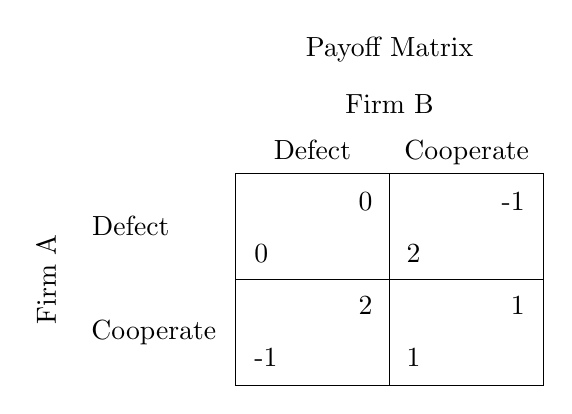
\begin{tikzpicture}

\matrix[matrix of math nodes,every odd row/.style={align=right},every even row/.style={align=left},every node/.style={text width=1.5cm},row sep=0.2cm,column sep=0.2cm] (m) {
0&-1\\
0&2\\
2&1\\
-1&1\\
};
\draw (m.north east) rectangle (m.south west);
\draw (m.north) -- (m.south);
\draw (m.east) -- (m.west);

\coordinate (a) at ($(m.north west)!0.25!(m.north east)$);
\coordinate (b) at ($(m.north west)!0.75!(m.north east)$);
\node[above=5pt of a,anchor=base] {Defect};
\node[above=5pt of b,anchor=base] {Cooperate};

\coordinate (c) at ($(m.north west)!0.25!(m.south west)$);
\coordinate (d) at ($(m.north west)!0.75!(m.south west)$);
\node[left=20pt of c,align=center,text width=1cm]  {Defect};
\node[left=20pt of d,align=center,text width=1cm]  {Cooperate};

\node[above=18pt of m.north,align=center] (firm b) {Firm B};
\node[left=2.4cm of m.west,rotate=90,align=center,anchor=center] {Firm A};

\node[above=5pt of firm b]  {Payoff Matrix};
\end{tikzpicture}

\begin{lstlisting}
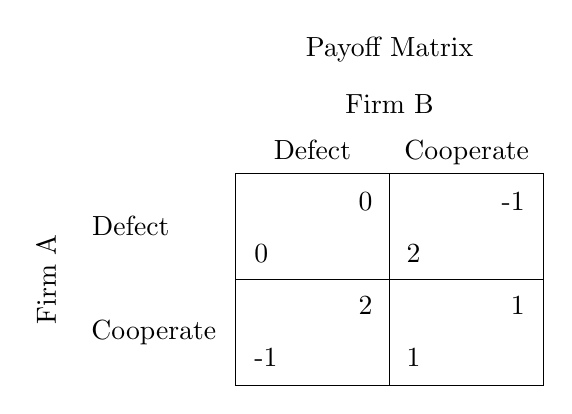
\begin{tikzpicture}
\matrix[matrix of math nodes,every odd row/.style={align=right},every even row/.style={align=left},every node/.style={text width=1.5cm},row sep=0.2cm,column sep=0.2cm] (m) {
0&-1\\
0&2\\
2&1\\
-1&1\\
};
\draw (m.north east) rectangle (m.south west);
\draw (m.north) -- (m.south);
\draw (m.east) -- (m.west);

\coordinate (a) at ($(m.north west)!0.25!(m.north east)$);
\coordinate (b) at ($(m.north west)!0.75!(m.north east)$);
\node[above=5pt of a,anchor=base] {Defect};
\node[above=5pt of b,anchor=base] {Cooperate};

\coordinate (c) at ($(m.north west)!0.25!(m.south west)$);
\coordinate (d) at ($(m.north west)!0.75!(m.south west)$);
\node[left=20pt of c,align=center,text width=1cm]  {Defect};
\node[left=20pt of d,align=center,text width=1cm]  {Cooperate};

\node[above=18pt of m.north,align=center] (firm b) {Firm B};
\node[left=2.4cm of m.west,rotate=90,align=center,anchor=center] {Firm A};

\node[above=5pt of firm b]  {Payoff Matrix};
\end{tikzpicture}
\end{lstlisting}




%%%%%%%%%%%%%%%%%%%%%%%%%%%%%%%%%%%%%%%%%%%%%%%%%%%%%%%%%%
%%%%%%%%%%%%%%%%%%%%%%%%%%%%%%%%%%%%%%%%%%%%%%%%%%%%%%%%%%




\subsubsection{Probability Tree}
This \emph{TikZ} graphic uses the \emph{inputenc} package, as well as the \emph{trees} library within \emph{TikZ}.  
{
%%%%%%%%%%%%%%%%%%%%%%%%%%%%%%%%%%%%%%%%%%%%%%%%%%%%%

% HEADER MATERIAL
%\usepackage[latin1]{inputenc}
%\usepackage{tikz}
%\usetikzlibrary{trees}
%\usepackage{verbatim}
% END HEADER MATERIAL

% Set the overall layout of the tree
\tikzstyle{level 1}=[level distance=3.5cm, sibling distance=3.5cm]
\tikzstyle{level 2}=[level distance=3.5cm, sibling distance=2cm]

% Define styles for bags and leafs
\tikzstyle{bag} = [text width=4em, text centered]
\tikzstyle{end} = [circle, minimum width=3pt,fill, inner sep=0pt]

% The sloped option gives rotated edge labels. Personally
% I find sloped labels a bit difficult to read. Remove the sloped options
% to get horizontal labels. 
\begin{tikzpicture}[grow=right, sloped]
\node[bag] {Bag 1 $4W, 3B$}
    child {
        node[bag] {Bag 2 $4W, 5B$}        
            child {
                node[end, label=right:
                    {$P(W_1\cap W_2)=\frac{4}{7}\cdot\frac{4}{9}$}] {}
                edge from parent
                node[above] {$W$}
                node[below]  {$\frac{4}{9}$}
            }
            child {
                node[end, label=right:
                    {$P(W_1\cap B_2)=\frac{4}{7}\cdot\frac{5}{9}$}] {}
                edge from parent
                node[above] {$B$}
                node[below]  {$\frac{5}{9}$}
            }
            edge from parent 
            node[above] {$W$}
            node[below]  {$\frac{4}{7}$}
    }
    child {
        node[bag] {Bag 2 $3W, 6B$}        
        child {
                node[end, label=right:
                    {$P(B_1\cap W_2)=\frac{3}{7}\cdot\frac{3}{9}$}] {}
                edge from parent
                node[above] {$B$}
                node[below]  {$\frac{3}{9}$}
            }
            child {
                node[end, label=right:
                    {$P(B_1\cap B_2)=\frac{3}{7}\cdot\frac{6}{9}$}] {}
                edge from parent
                node[above] {$W$}
                node[below]  {$\frac{6}{9}$}
            }
        edge from parent         
            node[above] {$B$}
            node[below]  {$\frac{3}{7}$}
    };
\end{tikzpicture}
}

\begin{lstlisting}
% Set the overall layout of the tree
\tikzstyle{level 1}=[level distance=3.5cm, sibling distance=3.5cm]
\tikzstyle{level 2}=[level distance=3.5cm, sibling distance=2cm]

% Define styles for bags and leafs
\tikzstyle{bag} = [text width=4em, text centered]
\tikzstyle{end} = [circle, minimum width=3pt,fill, inner sep=0pt]

% The sloped option gives rotated edge labels. Personally
% I find sloped labels a bit difficult to read. Remove the sloped options
% to get horizontal labels. 
\begin{tikzpicture}[grow=right, sloped]
\node[bag] {Bag 1 $4W, 3B$}
    child {
        node[bag] {Bag 2 $4W, 5B$}        
            child {
                node[end, label=right:
                    {$P(W_1\cap W_2)=\frac{4}{7}\cdot\frac{4}{9}$}] {}
                edge from parent
                node[above] {$W$}
                node[below]  {$\frac{4}{9}$}
            }
            child {
                node[end, label=right:
                    {$P(W_1\cap B_2)=\frac{4}{7}\cdot\frac{5}{9}$}] {}
                edge from parent
                node[above] {$B$}
                node[below]  {$\frac{5}{9}$}
            }
            edge from parent 
            node[above] {$W$}
            node[below]  {$\frac{4}{7}$}
    }
    child {
        node[bag] {Bag 2 $3W, 6B$}        
        child {
                node[end, label=right:
                    {$P(B_1\cap W_2)=\frac{3}{7}\cdot\frac{3}{9}$}] {}
                edge from parent
                node[above] {$B$}
                node[below]  {$\frac{3}{9}$}
            }
            child {
                node[end, label=right:
                    {$P(B_1\cap B_2)=\frac{3}{7}\cdot\frac{6}{9}$}] {}
                edge from parent
                node[above] {$W$}
                node[below]  {$\frac{6}{9}$}
            }
        edge from parent         
            node[above] {$B$}
            node[below]  {$\frac{3}{7}$}
    };
\end{tikzpicture}
\end{lstlisting}




%%%%%%%%%%%%%%%%%%%%%%%%%%%%%%%%%%%%%%%%%%%%%%%%%%%%%%%%%%
%%%%%%%%%%%%%%%%%%%%%%%%%%%%%%%%%%%%%%%%%%%%%%%%%%%%%%%%%%




\subsubsection{Red-Black Tree}
This image uses the \emph{verbatim} package to comment out blocks of text with notes describing the image.  It also uses the \emph{arrows} library in \emph{TikZ}.
{
%%%%%%%%%%%%%%%%%%%%%%%%%%%%%%%%%%%%%%%%%%%%%%%%%%%%%
% Author: Madit

% HEADER MATERIAL
%\usepackage{tikz}
%\usepackage{verbatim}
% END HEADER MATERIAL

\begin{comment}
:Author: Madit
A red-black tree is a special type of binary tree, used in computer science
to organize pieces of comparable data, such as text fragments or numbers.
(Wikipedia)
\end{comment}

\tikzset{
  treenode/.style = {align=center, inner sep=0pt, text centered,
    font=\sffamily},
  arn_n/.style = {treenode, circle, white, font=\sffamily\bfseries, draw=black,
    fill=black, text width=1.5em},% arbre rouge noir, noeud noir
  arn_r/.style = {treenode, circle, red, draw=red, 
    text width=1.5em, very thick},% arbre rouge noir, noeud rouge
  arn_x/.style = {treenode, rectangle, draw=black,
    minimum width=0.5em, minimum height=0.5em}% arbre rouge noir, nil
}

\begin{tikzpicture}[->,>=stealth',level/.style={sibling distance = 5cm/#1,
  level distance = 1.5cm}] 
\node [arn_n] {33}
    child{ node [arn_r] {15} 
            child{ node [arn_n] {10} 
            	child{ node [arn_r] {5} edge from parent node[above left]
                         {$x$}} %for a named pointer
							child{ node [arn_x] {}}
            }
            child{ node [arn_n] {20}
							child{ node [arn_r] {18}}
							child{ node [arn_x] {}}
            }                            
    }
    child{ node [arn_r] {47}
            child{ node [arn_n] {38} 
							child{ node [arn_r] {36}}
							child{ node [arn_r] {39}}
            }
            child{ node [arn_n] {51}
							child{ node [arn_r] {49}}
							child{ node [arn_x] {}}
            }
		}
; 
\end{tikzpicture}
}

\begin{lstlisting}
\begin{comment}
:Author: Madit
A red-black tree is a special type of binary tree, used in computer science to organize pieces of comparable data, such as text fragments or numbers.  (Wikipedia)
\end{comment}

\tikzset{
  treenode/.style = {align=center, inner sep=0pt, text centered,
    font=\sffamily},
  arn_n/.style = {treenode, circle, white, font=\sffamily\bfseries, draw=black,
    fill=black, text width=1.5em},% arbre rouge noir, noeud noir
  arn_r/.style = {treenode, circle, red, draw=red, 
    text width=1.5em, very thick},% arbre rouge noir, noeud rouge
  arn_x/.style = {treenode, rectangle, draw=black,
    minimum width=0.5em, minimum height=0.5em}% arbre rouge noir, nil
}

\begin{tikzpicture}[->,>=stealth',level/.style={sibling distance = 5cm/#1,
  level distance = 1.5cm}] 
\node [arn_n] {33}
    child{ node [arn_r] {15} 
            child{ node [arn_n] {10} 
              child{ node [arn_r] {5} edge from parent node[above left]
                         {$x$}} %for a named pointer
					child{ node [arn_x] {}}
            }
            child{ node [arn_n] {20}
					child{ node [arn_r] {18}}
					child{ node [arn_x] {}}
            }                            
    }
    child{ node [arn_r] {47}
            child{ node [arn_n] {38} 
					child{ node [arn_r] {36}}
					child{ node [arn_r] {39}}
            }
            child{ node [arn_n] {51}
					child{ node [arn_r] {49}}
					child{ node [arn_x] {}}
            }
		}
; 
\end{tikzpicture}
\end{lstlisting}




%%%%%%%%%%%%%%%%%%%%%%%%%%%%%%%%%%%%%%%%%%%%%%%%%%%%%%%%%%
%%%%%%%%%%%%%%%%%%%%%%%%%%%%%%%%%%%%%%%%%%%%%%%%%%%%%%%%%%




\subsubsection{H-tree and B-tree}
Here are two images side-by-side.  The vast majority of the code in this subsection is dedicated to defining the commands which ultimately produce the final diagrams in the final lines of code!  
{
%%%%%%%%%%%%%%%%%%%%%%%%%%%%%%%%%%%%%%%%%%%%%%%%%%%%%%%
% Author: Andrew Stacey

% BEGIN HEADER MATERIAL
%\usepackage{tikz}
%\usepackage{verbatim}
% END HEADER MATERIAL

\tikzset{
  htree leaves/.initial=2,
  sibling angle/.initial=20,
  htree level/.initial={}
}

\makeatletter

\def\htree@growth{%
  \pgftransformrotate{%
    (\pgfkeysvalueof{/tikz/sibling angle})*(-.5-.5*\tikznumberofchildren
      +\tikznumberofcurrentchild)}%
  \pgftransformxshift{\the\tikzleveldistance}%
  \pgfkeysvalueof{/tikz/htree level}%
}
\tikzstyle{htree}=[
  growth function=\htree@growth,
  sibling angle=180,
  htree level={
    \tikzleveldistance=.707\tikzleveldistance
    \pgfsetlinewidth{.707*\the\pgflinewidth}
  }
]

\tikzstyle{btree}=[
  growth function=\htree@growth,
  sibling angle=60,
  htree level={
    \tikzleveldistance=.55\tikzleveldistance
    \pgfsetlinewidth{.707*\the\pgflinewidth}
  }
]

\long\def\ge@addto@macro#1#2{%
  \begingroup
  \toks@\expandafter\expandafter\expandafter{\expandafter#1#2}%
  \xdef#1{\the\toks@}%
  \endgroup}

\newcommand{\htree}[2][]{%
  \def\htree@start{\noexpand\coordinate}
  \def\htree@end{}
  \foreach \l in {0,...,#2} {
    \g@addto@macro\htree@start{child foreach \noexpand\x in {1,2} {\iffalse}\fi}
    \g@addto@macro\htree@end{\iffalse{\fi}}
    \global\let\htree@start\htree@start
    \global\let\htree@end\htree@end
  }
  \edef\htree@cmd{\htree@start\htree@end;}
  \begin{scope}[htree,#1]
  \htree@cmd
  \end{scope}
}

\makeatother

\begin{tikzpicture}[
  rotate=90,
  yscale=.5,
  level distance=3cm,
  line width=8pt,
]
\htree{4}
\htree[btree,yshift=-12cm,xshift=-3cm]{7}
\end{tikzpicture}
}

\begin{lstlisting}
\tikzset{
  htree leaves/.initial=2,
  sibling angle/.initial=20,
  htree level/.initial={}
}

\makeatletter

\def\htree@growth{%
  \pgftransformrotate{%
    (\pgfkeysvalueof{/tikz/sibling angle})*(-.5-.5*\tikznumberofchildren
      +\tikznumberofcurrentchild)}%
  \pgftransformxshift{\the\tikzleveldistance}%
  \pgfkeysvalueof{/tikz/htree level}%
}
\tikzstyle{htree}=[
  growth function=\htree@growth,
  sibling angle=180,
  htree level={
    \tikzleveldistance=.707\tikzleveldistance
    \pgfsetlinewidth{.707*\the\pgflinewidth}
  }
]

\tikzstyle{btree}=[
  growth function=\htree@growth,
  sibling angle=60,
  htree level={
    \tikzleveldistance=.55\tikzleveldistance
    \pgfsetlinewidth{.707*\the\pgflinewidth}
  }
]

\long\def\ge@addto@macro#1#2{%
  \begingroup
  \toks@\expandafter\expandafter\expandafter{\expandafter#1#2}%
  \xdef#1{\the\toks@}%
  \endgroup}

\newcommand{\htree}[2][]{%
  \def\htree@start{\noexpand\coordinate}
  \def\htree@end{}
  \foreach \l in {0,...,#2} {
    \g@addto@macro\htree@start{child foreach \noexpand\x in {1,2} {\iffalse}\fi}
    \g@addto@macro\htree@end{\iffalse{\fi}}
    \global\let\htree@start\htree@start
    \global\let\htree@end\htree@end
  }
  \edef\htree@cmd{\htree@start\htree@end;}
  \begin{scope}[htree,#1]
  \htree@cmd
  \end{scope}
}

\makeatother

\begin{tikzpicture}[
  rotate=90,
  yscale=.5,
  level distance=3cm,
  line width=8pt,
]
\htree{4}
\htree[btree,yshift=-12cm,xshift=-3cm]{7}
\end{tikzpicture}
\end{lstlisting}




%%%%%%%%%%%%%%%%%%%%%%%%%%%%%%%%%%%%%%%%%%%%%%%%%%%%%%%%%%
%%%%%%%%%%%%%%%%%%%%%%%%%%%%%%%%%%%%%%%%%%%%%%%%%%%%%%%%%%




\subsubsection{Mindmap and Layers}
Finally, this complicated diagram is useful for visualizing the relationship between divergent concepts.  It also looks really cool.  It uses the \emph{times} package in addition to \emph{TikZ} and the \emph{TikZ} libraries, \emph{mindmap} and \emph{backgrounds}.  
{
%%%%%%%%%%%%%%%%%%%%%%%%%%%%%%%%%%%%%%%%%%%%%%%%%%%%%%%%%%%%%%%%%%%%%%%%
% Author  : Andrei Sobolevski (April 2009)
% License : Creative Commons attribution license

%HEADER MATERIAL
%\usepackage{verbatim}
%\usepackage{tikz,times}
%END HEADER MATERIAL

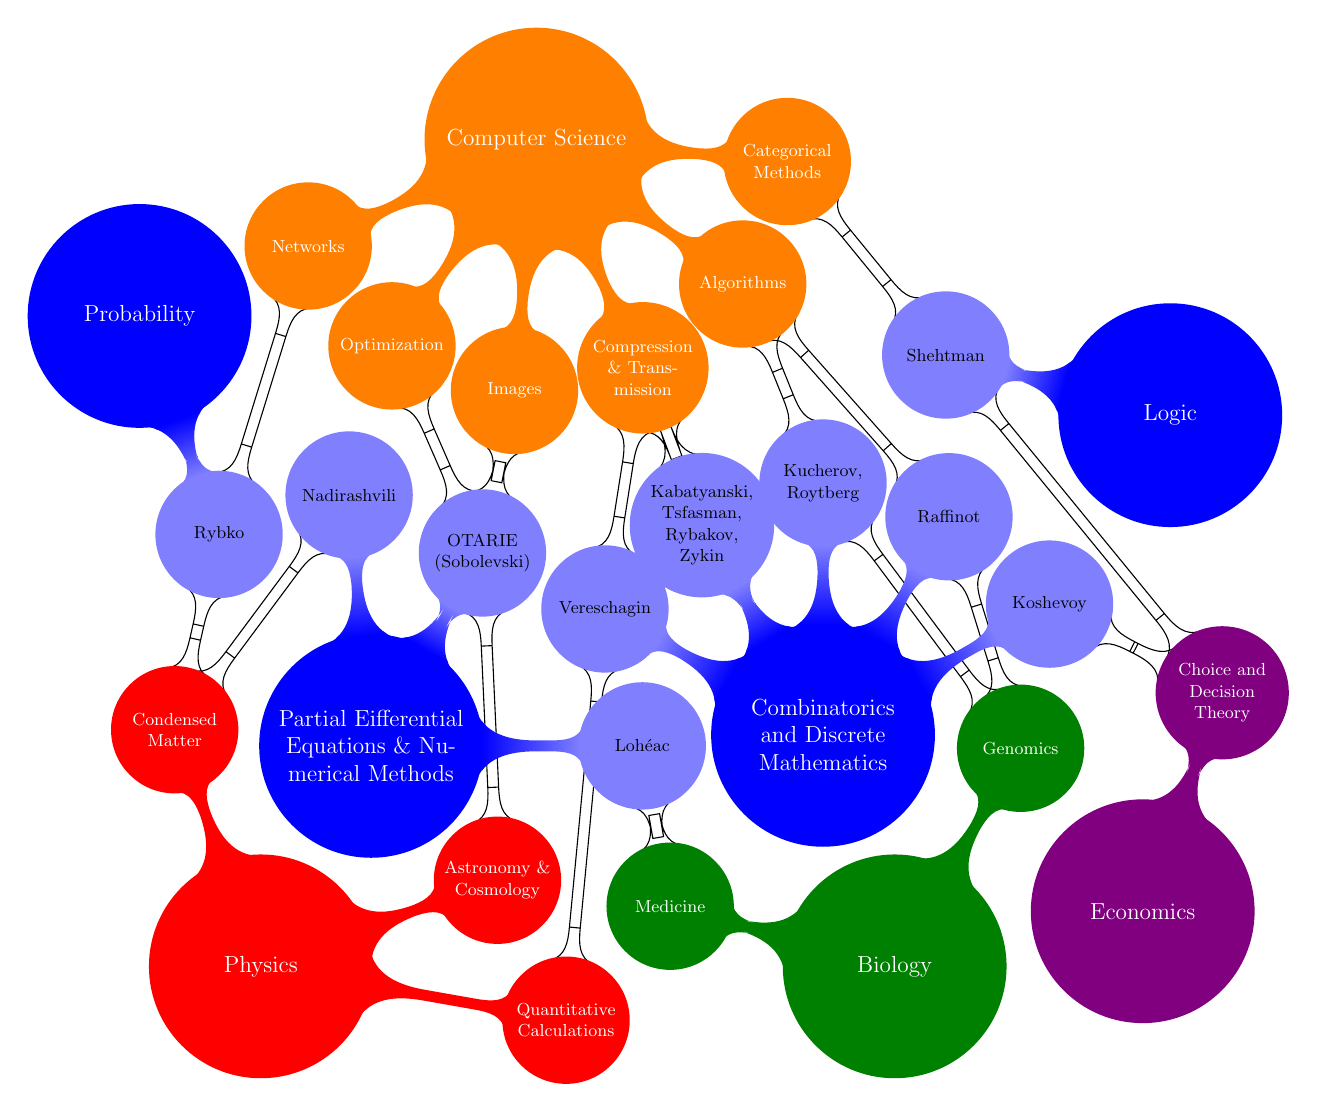
\begin{tikzpicture}[mindmap,
  level 1 concept/.append style={level distance=130,sibling angle=30},
  extra concept/.append style={color=blue!50,text=black},transform shape,scale=.7]

  % Applied area: computer science and its subfields
  \begin{scope}[mindmap, concept color=orange, text=white]
    \node [concept] {Computer Science}[clockwise from=-5] 
      child {node [concept] (log) {Categorical Methods}}
      child {node [concept] (alg) {Algorithms}}
      child {node [concept] (cod) {Compression \& Transmission}}
      child {node [concept] (img) {Images}}
      child {node [concept] (opt) {Optimization}}
      child {node [concept] (res) {Networks}};
  \end{scope}

  % Applied area: theoretical physics and its subfields
  \begin{scope}[mindmap, concept color=red,text=white]
    \node [concept] at (-5,-15) {Physics}
      child [grow=-10, level distance=160]
        {node [concept] (qin) {Quantitative Calculations}}
      child [grow=20] 
        {node [concept] (csm) {Astronomy \& Cosmology}}
      child [grow=110] 
        {node [concept] (mat) {Condensed Matter}};
  \end{scope}

  % Applied area: biology and its subfields
  \begin{scope}[mindmap, concept color=green!50!black,text=white]
    \node [concept] at (6.5,-15) {Biology} 
      child [grow=165, level distance=120] 
        {node [concept] (med) {Medicine}}
      child [grow=60] 
        {node [concept] (gen) {Genomics}};
  \end{scope}

  % Applied area: economics (one subfield)
  \begin{scope}[mindmap, concept color=violet, text=white]
    \node [concept] at (11,-14) {Economics}
      child [grow=70, level distance=120] 
        {node [concept] (dec) {Choice and Decision Theory}};
  \end{scope}

  % Researchers listed by their main specialization in mathematics

  \begin{scope}[mindmap, concept color=blue]

    % Combinatorics and discrete mathematics 
    \node [concept, text=white] at (5.2,-10.8) 
      {Combinatorics and Discrete Mathematics} 
      [clockwise from=150]
      child [concept color=blue!50] {node [concept] (ver) {Vereschagin}}
      child [concept color=blue!50, level distance=125] 
        {node [concept] (kab) {Kabatyanski, Tsfasman, Rybakov, Zykin}}
      child [concept color=blue!50] 
        {node [concept] (kch) {Kucherov, Roytberg}}
      child [concept color=blue!50] {node [concept] (raf) {Raffinot}}
      child [concept color=blue!50, level distance=135]
        {node [concept] (ksh) {Koshevoy}};

    % Partial differential equations
    \node [concept, text=white] at (-3,-11) 
      {Partial Eifferential Equations 
        \& Numerical Methods}
      child [concept color=blue!50, grow=0, level distance=140] 
        {node [concept] (lhc) {Loh{\'e}ac}}
      child [concept color=blue!50, grow=60, level distance=115] 
        {node [concept] (otr) {OTARIE (Sobolevski)}}
      child [concept color=blue!50, grow=95] {node [concept] (ndr) 
        {Nadirashvili}};

    % Probability
    \node [concept, text=white] at (-7.2,-3.2) {Probability}
      child [concept color=blue!50, grow=-70, level distance=120] 
        {node [concept] (rbk) {Rybko}};

    % Logic
    \node [concept, text=white] at (11.5,-5) {Logic}
      child [concept color=blue!50, grow=165, level distance=120] 
        {node [concept] (sht) {Shehtman}};
  \end{scope}

  % Connections of researchers to applied subfields

  \begin{pgfonlayer}{background}
    \draw [circle connection bar]
      (kab) edge (cod)
      (kch) edge (alg) edge (gen)
      (lhc) edge (med)
      (ksh) edge (dec)
      (ndr) edge (mat)
      (otr) edge (opt) edge (csm) edge (img)
      (raf) edge (alg) edge (gen)
      (rbk) edge (res) edge (mat)
      (sht) edge (log) edge (dec)
      (ver) edge (qin) edge (cod);
  \end{pgfonlayer}
\end{tikzpicture}
}

\begin{lstlisting}
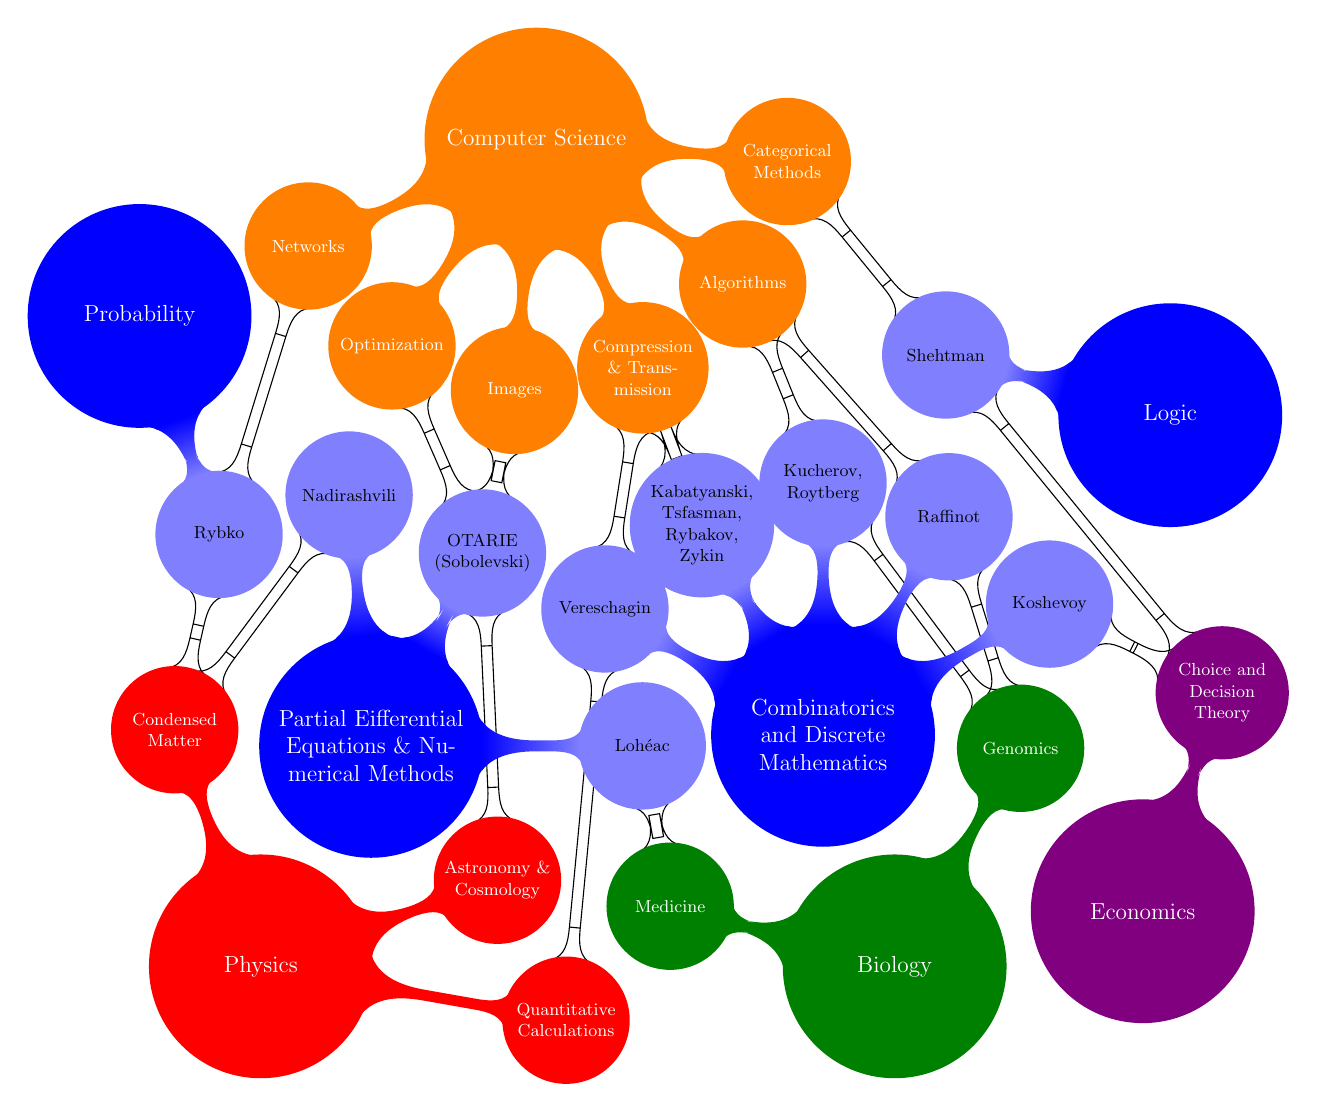
\begin{tikzpicture}[mindmap,
  level 1 concept/.append style={level distance=130,sibling angle=30},
  extra concept/.append style={color=blue!50,text=black},transform shape,scale=.7]

  % Applied area: computer science and its subfields
  \begin{scope}[mindmap, concept color=orange, text=white]
    \node [concept] {Computer Science}[clockwise from=-5] 
      child {node [concept] (log) {Categorical Methods}}
      child {node [concept] (alg) {Algorithms}}
      child {node [concept] (cod) {Compression \& Transmission}}
      child {node [concept] (img) {Images}}
      child {node [concept] (opt) {Optimization}}
      child {node [concept] (res) {Networks}};
  \end{scope}

  % Applied area: theoretical physics and its subfields
  \begin{scope}[mindmap, concept color=red,text=white]
    \node [concept] at (-5,-15) {Physics}
      child [grow=-10, level distance=160]
        {node [concept] (qin) {Quantitative Calculations}}
      child [grow=20] 
        {node [concept] (csm) {Astronomy \& Cosmology}}
      child [grow=110] 
        {node [concept] (mat) {Condensed Matter}};
  \end{scope}

  % Applied area: biology and its subfields
  \begin{scope}[mindmap, concept color=green!50!black,text=white]
    \node [concept] at (6.5,-15) {Biology} 
      child [grow=165, level distance=120] 
        {node [concept] (med) {Medicine}}
      child [grow=60] 
        {node [concept] (gen) {Genomics}};
  \end{scope}

  % Applied area: economics (one subfield)
  \begin{scope}[mindmap, concept color=violet, text=white]
    \node [concept] at (11,-14) {Economics}
      child [grow=70, level distance=120] 
        {node [concept] (dec) {Choice and Decision Theory}};
  \end{scope}

  % Researchers listed by their main specialization in mathematics

  \begin{scope}[mindmap, concept color=blue]

    % Combinatorics and discrete mathematics 
    \node [concept, text=white] at (5.2,-10.8) 
      {Combinatorics and Discrete Mathematics} 
      [clockwise from=150]
      child [concept color=blue!50] {node [concept] (ver) {Vereschagin}}
      child [concept color=blue!50, level distance=125] 
        {node [concept] (kab) {Kabatyanski, Tsfasman, Rybakov, Zykin}}
      child [concept color=blue!50] 
        {node [concept] (kch) {Kucherov, Roytberg}}
      child [concept color=blue!50] {node [concept] (raf) {Raffinot}}
      child [concept color=blue!50, level distance=135]
        {node [concept] (ksh) {Koshevoy}};

    % Partial differential equations
    \node [concept, text=white] at (-3,-11) 
      {Partial Eifferential Equations 
        \& Numerical Methods}
      child [concept color=blue!50, grow=0, level distance=140] 
        {node [concept] (lhc) {Loh{\'e}ac}}
      child [concept color=blue!50, grow=60, level distance=115] 
        {node [concept] (otr) {OTARIE (Sobolevski)}}
      child [concept color=blue!50, grow=95] {node [concept] (ndr) 
        {Nadirashvili}};

    % Probability
    \node [concept, text=white] at (-7.2,-3.2) {Probability}
      child [concept color=blue!50, grow=-70, level distance=120] 
        {node [concept] (rbk) {Rybko}};

    % Logic
    \node [concept, text=white] at (11.5,-5) {Logic}
      child [concept color=blue!50, grow=165, level distance=120] 
        {node [concept] (sht) {Shehtman}};
  \end{scope}

  % Connections of researchers to applied subfields

  \begin{pgfonlayer}{background}
    \draw [circle connection bar]
      (kab) edge (cod)
      (kch) edge (alg) edge (gen)
      (lhc) edge (med)
      (ksh) edge (dec)
      (ndr) edge (mat)
      (otr) edge (opt) edge (csm) edge (img)
      (raf) edge (alg) edge (gen)
      (rbk) edge (res) edge (mat)
      (sht) edge (log) edge (dec)
      (ver) edge (qin) edge (cod);
  \end{pgfonlayer}
\end{tikzpicture}
\end{lstlisting}




%%%%%%%%%%%%%%%%%%%%%%%%%%%%%%%%%%%%%%%%%%%%%%%%%%%%%%%%%%
%%%%%%%%%%%%%%%%%%%%%%%%%%%%%%%%%%%%%%%%%%%%%%%%%%%%%%%%%%




\section{Conclusion}
Now that you have made it this far, it is time to just jump in and start playing around with the software.  Practice makes perfect, right?  If you have more requests for information to include, let me know.  I will try to update this document over time to add functionality as well as make the learning experience easier.  Hopefully there is enough here to at least give you an idea of what to look for as you attempt to write documents in \LaTeX.  

\bibliographystyle{jpe}

\nocite{*}

\hfill \today 

\bibliography{BiblioTemp}

\end{document}
